%%%%%%%%%%%%%%%%%%%%%%%%%%%%%%%%%%%%%%%%%%%%%%%%%%%%%%%%%
%                                                       %
% La clase: 11pt o 10pt, es un draft o copia definitiva %
% Que tipo de codificacion usa, ...                     %
%                                                       %
%%%%%%%%%%%%%%%%%%%%%%%%%%%%%%%%%%%%%%%%%%%%%%%%%%%%%%%%%
\documentclass[11pt,twoside,a4paper]{book}
\usepackage{fancyhdr}
\usepackage{fancybox}
\usepackage[T1]{fontenc}
\usepackage[utf8]{inputenc}
\usepackage[spanish]{babel}
\usepackage{mathptmx}
\usepackage{amsfonts}
\usepackage{latexsym}
\usepackage{graphicx}
\usepackage{floatflt}
\usepackage{float}
\usepackage{epsfig}
\usepackage{subfigure}
\usepackage{mathrsfs}
\usepackage{amssymb}
\renewcommand{\baselinestretch}{1.2}
\graphicspath{ {./images/} }
\title{\Huge Práctica 1 IAA}
\author{Daniel Ranchal Parrado, Francisco Vera Herencia}
\date{\parbox{\linewidth}{\centering%
  \today\endgraf\bigskip
  32 horas de trabajo}}
%%%%%%%%%%%%%%%%%%%%%%%%%%%
%                         %
% Comenzamos el documento %
%                         %
%%%%%%%%%%%%%%%%%%%%%%%%%%%
\begin{document}
\maketitle
%%%%%%%%%%%%%%%%%%%%%%%%%%%
%
% Algunos ajustes previos
%
%%%%%%%%%%%%%%%%%%%%%%%%%%%

\renewcommand\bibname{Bibliografía}
\renewcommand\tablename{Tabla}

\pagenumbering{arabic} \fancyhf{} \pagestyle{fancy}
\fancyhead[LO]{\rightmark} % En las pginas impares, parte izquierda del encabezado, aparecer el nombre de seccin
\fancyhead[RE]{\leftmark} % En las pginas pares, parte derecha del encabezado, aparecer el nombre de captulo
\fancyhead[RO,LE]{\thepage} % Nmeros de pgina en las esquinas de los encabezados
\setlength{\headheight}{14pt}
\renewcommand{\sectionmark}[1]{\markright{{\thesection. #1}}} % Formato para la seccin: N.M. Nombre

\tableofcontents
\listoffigures

\chapter{Primer ejercicio}
\section{¿Cuántos atributos caracterizan los datos de esta base de datos?}
Los datos se caracterizan por 5 atributos, como se puede apreciar en la figura \ref{Fig1}.
\begin{figure}[H]
   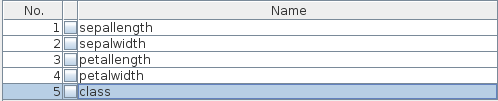
\includegraphics[width=\textwidth]{attributes.png}
   \caption{atributos}
   \label{Fig1}
\end{figure}

\section{¿Se trata de regresión o clasificación?}
Se trata de una clasificación, ya que a partir de unos atributos se puede decir \
que una instancia pertenece a una clase u a otra según los valores de estos atributos.

\section{¿Cuál es el rango de valores del atributo petalwidth?¿Y su media? ¿y su desviación típica?}
Respecto al rango de valores del atributo petalwidth (anchura del pétalo), vendrá \
dado por los valores mínimo y máximo registrado, por lo que, según la figura \
\ref{Fig2} este rango será [0'1,2'5]. En la misma imagen también se indica la media y su desviación típica, cuyos valores son  1'199 y 0'763, respectivamente.
\begin{figure}[H]
	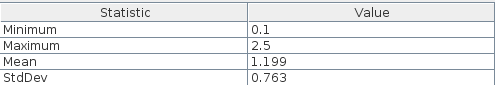
\includegraphics[width=\textwidth]{petalwidth.png}
	\caption{Rango, media y desviación típica de los datos del atributo petalwidth}
	\label{Fig2}
\end{figure}

\section{Determinar que atributo permite discriminar linealmente entre la clase iris-setosa y las otras dos clases}
\begin{figure}[H]
	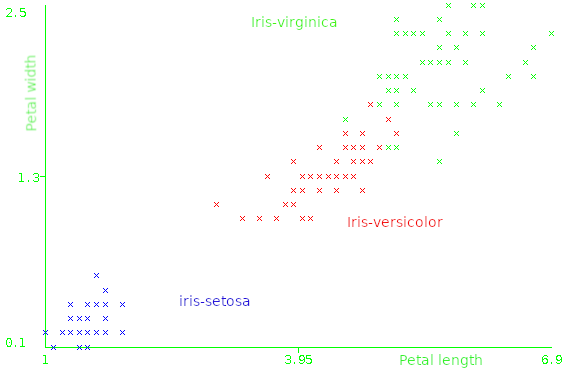
\includegraphics[width=\textwidth]{Plot.png}
	\caption{Gráfico en el que se diferencian las diferentes instancias según el ancho y la longitud del pétalo}
	\label{Fig3}
\end{figure}
Como se puede observer en la figura \ref{Fig3}, se puede diferenciar con bastante\
exactitud la clase iris-setosa y el resto de la clases. Para poder diferenciarlas de esta\
manera se han utiizado los atributos petallenght y petalwidth.

\section{Servicios y sus posibles resultados}
El servidor web Tomcat nos provee una gran cantidad de utilidades para \
aprovechar al máximo este mismo. La primera y la más importante es el despliegue\
de una página web. Tomcat nos permite hacerlo de manera estática, es decir, \
configurar la aplicación antes de activar este servicio o de manera dinámica, \
que es lo más utilizado para servidores que están en producción.
\newline
Para poder realizar esto de una manera sencilla, Tomcat nos da una herramienta \
llamada "Manager", que cómo se ha comentado antes, se pueden hacer despliegues \
y eliminación (undeploy) de cualquier aplicación web además de darnos una lista \
de las aplicaciones que ya están desplegadas.
\newline
Pero las utilidades de "Manager" no son sólo esas, este gestor nos da la opción \
de poder ver las estadísticas de las sesiones de cualquier aplicación y el \
estado del servidor. Otra de las funcionalidades que tiene, al igual que el \
servidor httpd y apache2, es la posibilidad de trabajar con "Virtual Host".
\newline
Otra característica interesante que nos ofrece Tomcat es la gestión de los \
usuario y los roles en las distintas aplicaciones web. Esto evita que tengamos \
una tabla para cada aplicación web que se tenga. En temas de seguridad, Tomcat \
nos permite la configuración de los certificados SSL/TLS para que nuestra \
página tenga el protocolo https.
\newline
Para este experimento, se distinguirán los siguientes resultados:

\begin{itemize}
  \item \textbf{La carga correcta de las imágenes en un tiempo\
  considerablemente bueno.}
  \item \textbf{La carga correcta de las imágenes en un tiempo pésimo.}
  \item \textbf{La carga parcial de las imágenes.}
  \item \textbf{Fallo del servidor web. Ninguna imágen es servida.}
\end{itemize}


\section{Métricas}
Para poder medir la eficacia y la actuación del servidor web Tomcat se han \
considerado los siguientes parámetros a examinar:

\begin{itemize}
  \item \textbf{Peticiones por segundo}
  \item \textbf{Tiempo por cada grupo de peticiones al mismo tiempo}
  \item \textbf{Tiempo por cada petición}
  \item \textbf{Uso de la CPU}
  \item \textbf{E/S Disco}
  \item \textbf{E/S Red}
\end{itemize}

\pagebreak
\section{Parámetros}
Los parámetros que pueden afectar a la medición del rendimiento del servidor \
web Tomcat son los siguientes:

\begin{itemize}
  \item \textbf{La lejanía con el centro de datos}
  \item \textbf{Los procesos que se ejecutan en segundo plano}
  \item \textbf{Estado de nuestra conexión a Internet}
  \item \textbf{Hardware empleado en el servidor}
\end{itemize}

Para poder mitigar los efectos que producen estos parámetros,la prueba se \
ejecutará varias veces y se harán los cáculos oportunos para representar de \
una manera correcta las estadísticas.

\chapter{Evaluación del Sistema}
Tras el montaje del servidor en Tomcat usando CentOS, procedemos a evaluar el\
sistema. En general hay muchas técnicas de evaluación posible. En nuestro caso\
vamos a realizar pruebas con Apache benchmark en el lado del cliente, y a \
monitorizar en el lado del servidor a través de sar y el monitor de Azure.\
Tras realizar esto, sacaremos los datos, tanto del lado del cliente como del\
servidor, y los analizaremos.

\section{Técnicas de evaluación}
Antes de proceder a describir los resultados, debemos mostrar cuáles fueron las\
técnicas utilizadas para obtener los resultados del benchmark. Para realizar\
estas pruebas, hemos hecho uso de Apache benchmark, debido a que es una de las \
principales utilidades a la hora de realizar benchmarking a un servidor web.\
Este permite mostrar pruebas con una concurrencia que nos sería difícil de\
imitar, además de sacar datos muy interesantes, como el tiempo medio de una\
petición y el número de peticiones del servidor.
Para sacar los datos hemos utilizado el monitor sar, realizando un monitoreo\
completo a la vez que sucedían las sucesivas pruebas de Apache benchmark. El\
monitor sar nos permite sacar datos, tanto de la utilización de CPU, como de\
red, además de otros muchos datos, los cuales no resaltaremos. Por último,\
hemos utilizado datos que nos dá el propio Azure a la hora de medir el uso de disco.


\section{Carga de trabajo}
Hemos hecho uso de tres cargas distintas de ab. Cada carga se ha realizado con \
una concurrencia y una cantidad de peticiones distintas, además de que cada una \
de estas se ha realizado en cinco ocasiones en tres index: uno con fotos \
grandes, otro con fotos medianas y otro con fotos pequeñas, para comprobar si \
existen diferencias entre las tres versiones. Las cargas son:
\begin{itemize}
  \item \textbf{ab -c 5 -n 20}: Pretende medir la capacidad  del programa a la \
  hora de tener una concurrencia media y una cantidad de peticiones \
  moderada/alta.
  \item \textbf{ab -c 1 -n 10}: Pretende probar el servidor con una cantidad \
  de peticiones más baja que la anterior prueba, pero sin concurrencia, para \
  comprobar la diferencia entre una prueba con concurrencia o sin ella.
  \item \textbf{ab -c 10 -t 40 -s 40}: Pretende probar el servidor con una \
  concurrencia alta en un tiempo, dándonos, por ejemplo, el número de \
  peticiones que puede realizar el servidor en x segundos.
\end{itemize}

\section{Diseño de Experimentos}
Para realizar estos experimentos he creado un script que realiza en cinco\
ocasiones las pruebas anteriormente nombradas para cada tamaño de imagen. A su \
vez, el monitor sar está corriendo en el servidor y guardándolo en un fichero.\
Para mostrar gráficamente los resultados de estas pruebas se hace uso de gnuplot.

\section{Análisis de los resultados}
Tras realizar ab y a los tres index con las distintas cargas podemos proceder a\
mostrar sus datos. Los primeros datos que nos resultarían interesantes serían\
los del propio Apache benchmark.
Los primeros datos que podemos mirar son los que nos da el propio apache\
benchmark. Estos datos, obtenidos de la propia salida del comando “ab” son \
los siguientes. De la primera prueba se extrae lo siguiente:

\begin{center}
\small
\begin{tabular}{ |c|c|c|c|c|c|c|c|c|c| }
 \hline
  & \multicolumn{3}{|c}{Pequeños} & \multicolumn{3}{|c|}{Medianos} & \multicolumn{3}{|c|}{Grandes} \\
 \hline
 Ejecución & Pet/s & ms/Petición & Total(s) \
 & Pet/s & ms/Petición & Total(s) &\
 Pet/s & ms/Petición & Total(s) \\
 \hline
 1 & 0.17 & 28875.345 & 115.501 & 0.16 & 31396.260 & 125.585 & 0.18 & 27800.182 & 111.201 \\
 \hline
 2 & 0.17 & 29610.067 & 118.440 & 0.17 & 30268.598 & 121.074 & 0.18 & 27508.504 & 110.034 \\
 \hline
 3 & 0.17 & 29360.455 & 117.442 & 0.17 & 30065.704 & 120.263 & 0.18 & 27296.960 & 109.185 \\
 \hline
 4 & 0.17 & 29445.476 & 117.782 & 0.16 & 32097.834 & 128.391 & 0.18 & 27261.818 & 109.047 \\
 \hline
 5 & 0.16 & 28917.908 & 115.672 & 0.17 & 29742.525 & 118.970 & 0.18 & 26643.844 & 106.575 \\
 \hline
 Media & 0.168 & 29241.8502 & 116.9674 & 0.166 & 30714.1842 & 122.8566 & 0.188 & 27302.2616 & 109.2084 \\
 \hline
\end{tabular}
\end{center}

Es curioso el hecho de que la variación del tiempo no dependa tanto del tamaño \
como de la capacidad de la red en ese momento. Se puede ver que aunque en los \
valores medianos sube el tiempo, tanto por petición como el total, con respecto \
a los valores pequeños; en los grandes esta sube debido a que la red no está \
siendo utilizada. \newline

Tras la segunda prueba nos da los siguientes resultados:

\begin{center}
\small
\begin{tabular}{ |c|c|c|c|c|c|c|c|c|c| }
 \hline
  & \multicolumn{3}{|c}{Pequeños} & \multicolumn{3}{|c|}{Medianos} & \multicolumn{3}{|c|}{Grandes} \\
 \hline
 Ejecución & Pet/s & ms/Petición & Total(s) \
 & Pet/s & ms/Petición & Total(s) &\
 Pet/s & ms/Petición & Total(s) \\
 \hline
 1 & 0.17 & 5897.409 & 58.974 & 0.16 & 6207.914 & 62.079 & 0.17 & 5732.952 & 57.330 \\
 \hline
 2 & 0.17 & 5952.298 & 59.523 & 0.16 & 6166.424 & 61.664 & 0.17 & 5792.583 & 57.926 \\
 \hline
 3 & 0.17 & 5968.026 & 59.680 & 0.16 & 6159.262 & 61.593 & 0.17 & 5720.497 & 57.205 \\
 \hline
 4 & 0.16 & 6904.65 & 60.946 & 0.16 & 6291.626 & 62.916 & 0.17 & 5761.08 & 57.611 \\
 \hline
 5 & 0.17 & 6033.483 & 60.335 & 0.16 & 6239.134 & 62.391 & 0.17 & 5817.991 & 58.180 \\
 \hline
 Media & 0.168 & 5989.1642 & 59.8916 & 0.16 & 6212.8708 & 62.1286 & 0.17 & 5765.0206 & 57.6504 \\
 \hline
\end{tabular}
\end{center}

Se puede comprobar que el tiempo de respuesta en este caso, sin ninguna\break\
concurrencia, es sustancialmente menor al tiempo con concurrencia\
(de media, unas 4.853981 veces menor), debido a que con más de dos peticiones a\
la vez el servidor se satura debido a su baja capacidad de cómputo. \newline

Por último, en el último test, siendo los dos únicos datos que nos interesan\
la media de peticiones que son capaces de resolver en ese tiempo y el tiempo\
de respuesta por petición.

\begin{center}
\small
\begin{tabular}{ |c|c|c|c|c|c|c| }
 \hline
  & \multicolumn{2}{|c}{Pequeños} & \multicolumn{2}{|c|}{Medianos} & \multicolumn{2}{c|}{Grandes} \\
 \hline
 Ejecución & Pet. hechas & ms/Petición \
 & Pet. hechas & ms/Petición &\
 Pet. hechas & ms/Petición \\
 \hline
 1 & 4 & 88795.308 & 4 & 110129.467 & 2 & 218473.645 \\
 \hline
 2 & 3 & 107076.853 & 3 & 130129.422 & 3 & 157925.583 \\
 \hline
 3 & 4 & 86692.71 & 4 & 108129.467 & 4 & 110129.562 \\
 \hline
 4 & 5 & 66522.661 & 2 & 160291.622 & 3 & 142129.465 \\
 \hline
 5 & 3 & 108506.811 & 4 & 110129.467 & 4 & 100345.234 \\
 \hline
 Media & 3.8 & 75914.1808 & 3.4 & 123761.889 & 3.2 & 145800.6978 \\
 \hline
\end{tabular}
\end{center}

Aqui si se puede notar una clara diferencia entre la performance entre la\
versión pequeña, la mediana y la grande, así como la del tiempo de respuesta\
entre las distintas ejecuciones. La principal diferencia de esta prueba con\
respecto a las otras dos es que, además de ser de tiempo, también tiene una\
concurrencia alta, sobre todo teniendo en cuenta, como veremos posteriormente,\
que la cpu a partir de dos concurrencias llega casi al 100\% de utilización.

A continuación procedemos a sacar con sar -u los datos de la CPU que se han\
sacado durante las distintas ejecuciones de ab. Con gnuplot los ponemos de\
manera visual, siendo la abscisa Y el porcentaje de uso de cpu y la abscisa\
X el tiempo.

% \begin{figure}[H]
%    \includegraphics[width=\textwidth]{cpugrandes.jpg}
%    \caption{Uso de CPU con imágenes grandes}
%    \label{cpu1}
% \end{figure}

% \begin{figure}[H]
%    \includegraphics[width=\textwidth]{cpumedianos.jpg}
%    \caption{Uso de CPU con imágenes medianas}
%    \label{cpu2}
% \end{figure}
%
% \begin{figure}[H]
%    \includegraphics[width=\textwidth]{cpupequenos.jpg}
%    \caption{Uso de CPU con imágenes medianas}
%    \label{cpu3}
% \end{figure}
Lo primero que se puede notar es que para una concurrencia mayor que uno, el\
servidor utiliza la cpu casi al 100\%, siendo el único momento donde este uso\
baja, cuando llega el momento de la prueba 2, donde no hay concurrencia y\
solo utiliza un 80\% del disco. \newline
En cuanto a las pruebas de red, he utilizado sar -n DEV para comprobar todos\
los paquetes que se han enviado. Además de esto, he usado sar -n EDEV para\
comprobar aquellos paquetes que no han sido recibidos, dando como resultado\
que en ninguna de las pruebas ha habido paquetes fallidos. Para mostrar los\
resultados, he vuelto a hacer uso de gnuplot, siendo la abscisa Y los kbs,\
tanto transmitidos como recibidos, y la abscisa X el tiempo.
% \begin{figure}[H]
%    \includegraphics[width=\textwidth]{redgrandes.jpg}
%    \caption{Uso de Red con imágenes grandes}
%    \label{red1}
% \end{figure}

% \begin{figure}[H]
%    \includegraphics[width=\textwidth]{redmedianos.jpg}
%    \caption{Uso de Red con imágenes medianas}
%    \label{red2}
% \end{figure}
%
% \begin{figure}[H]
%    \includegraphics[width=\textwidth]{redpequenos.jpg}
%    \caption{Uso de Red con imágenes pequeñas}
%    \label{red3}
% \end{figure}
Se puede notar como el ritmo de transferencia da muchas subidas y bajadas.\
Aun así los datos son más o menos estables, siendo el punto en el que es más\
baja la transferencia durante el tercer test, mientras que el punto en el que\
alcanza sus picos es en el segundo test. \newline
Por último, haciendo uso del monitor de azure y sacando media de los datos\
durante las ejecuciones de los benchmark, podemos sacar los datos de\
utilización de disco. Para mostrar estos datos, se ha hecho uso del\
excel, mostrando en ese caso la media por ejecución.

% \begin{figure}[H]
%    \includegraphics[width=\textwidth]{grafica2.jpg}
%    \caption{Uso de disco en las cinco ejecuciones con imágenes grandes}
%    \label{Fig2}
% \end{figure}
%
% \begin{figure}[H]
%    \includegraphics[width=\textwidth]{grafica3.jpg}
% \caption{Uso de disco en las cinco ejecuciones con imágenes medianas}   \label{Fig3}
% \end{figure}
%
% \begin{figure}[H]
%    \includegraphics[width=\textwidth]{grafica4.jpg}
%    \caption{Uso de disco en las cinco ejecuciones con imágenes pequeñas}
%    \label{Fig4}
% \end{figure}
Se pueden ver como las transferencias son muy parecidas, tanto entre benchmark\
como entre los distintos index.

\chapter{Conclusiones y discusión}

En primer lugar, se aprecia un fuerte problema en el hardware de este servidor \
debido al cuello de botella que aparece al ejecutar los bencharmarks en la CPU, \
esto es fácil de comprender, debido a que la concurrencia toma protagonismo en \
estos tests, con algunos fijándola en valores como 10 peticiones concurrentes. \
Esta teoría es afirmada por las gráficas mostradas, donde vemos fácilmente como \
el procesador llega a funcionar a niveles cercanos al 100\% de utilidad durante \
la duración de las pruebas efectuadas.\newline \newline
\indent Además de esto, otro factor determinante en este caso es el bajo número de \
transferencias por segundo que el servidor es capaz de aguantar y que está \
fuertemente relacionado con el almacenamiento del mismo en el cual se almacenan \
las fotografías que sirven como cargas de prueba, el cual en ninguna prueba es \
capaz de llegar ni tan siquiera a la unidad, y eso es algo que los encargados \
de testear su funcionamiento hemos conocido de primera mano al tener que \
esperar grandes cantidades de tiempo a que todos los tests fueran completados \
varias veces con éxito. En cuanto a las peticiones por segundo, casi nunca \
superan el cuarto de unidad, hecho que no hace más que corroborar las \
afirmaciones anteriores. \newline

% \begin{figure}[H]
%    \includegraphics[width=\textwidth]{grafica1.jpg}
%    \caption{Transferencias por Segundo, peticiones por segundo \
%    y tiempo empleado en un grupo de peticiones concurrentes.}
%    \label{Fig1}
% \end{figure}

Si contemplamos el gráfico pipo, nos damos cuenta de que el número de \
peticiones por segundo, al ser un parámetro íntimamente ligado al hardware \
sobre el que se esté ejecutando el banco de pruebas escogido, apenas varía, \
puesto que la CPU solo es capaz de ejecutar un número determinado de ellas, \
siendo todas iguales. Lo interesante de este gráfico, es ver como el tiempo \
empleado en servir un grupo de peticiones concurrentes decae a lo largo de las \
cinco ejecuciones del test. Tras indagar en los motivos de este aumento del \
rendimiento, nos damos cuenta de que Azure es un servicio de computación en la \
nube que alardea de proveer de una caché inteligente a sus máquinas virtuales \
que estén corriendo en sus servidores, como es nuestro caso, eso por ello por \
lo que se aprecia esta mejora en el rendimiento, debido a que gran parte de los \
datos que son necesarios para la ejecución de la prueba, ya están cargados en \
la caché del servidor y son accesibles de manera mucho más rápida para la \
siguiente ejecución. \newline \newline
% \indent Si contemplamos las gráficas \ref{Fig2}, \ref{Fig3} y \ref{Fig4}, no hay gran \
diferencia entre ellas en cuanto al parámetro de medición, el número de \
transferencias por segundo del disco del servidor. Para analizar las gráficas, \
recordemos que estos datos han sido tomados con el monitor sar, mientras que ab \
era ejecutado, tras ello, se ha realizado la media aritmética de los valores \
del parámetro interesado que sar tomaba cada 10 segundos durante la ejecución \
del test. Entonces, podemos ver como apenas hay diferencias significativas \
% entre las ejecuciones, por ejemplo, en la gráfica \ref{Fig2}, vemos como\
normalmente el test de menor concurrencia y menos repeticiones\
(línea amarilla), tarda normalmente menos tiempo que el test con más \
concurrencia y el doble de repeticiones (línea verde), aunque veamos \
ejecuciones donde estas posiciones se inviertan, esto se debe más al margen de \
% error que a otra cosa. En cuanto a la gráfica \ref{Fig4}, la referida a los \
resultados del mosaico de imágenes pequeñas, observamos como la línea azul, \
la correspondiente con el uso de https, lo cual es curioso debido a que en las \
dos últimas pruebas se habían mantenido por debajo, sin embargo, no es de \
preocupación, ya que no se aprecian diferencias muy significativas en la \
mayoría de las ejecuciones, sin embargo, vemos como esa línea sube hasta una \
transferencia por segundo en la segunda ejecución, lo cual es muy significativo.
La imagen general de estas pruebas es que mientras más grandes sean las \
imágenes del banco de pruebas, menos transferencias por segundo se llevarán a \
cabo, lo cual es lógico, puesto que son archivos más grandes. \newline
Si analizamos ahora el uso de la red del servidor, aquí no tenemos ningún \
problema de cuello de botella, Azure nos proporciona una velocidad de conexión \
veloz y estable y no es algo que un administrador de un servidor pequeño como \
este tenga que preocuparse, por supuesto, mientras más exigente sea el test con \
la CPU, lo será con el uso de red que éste requerirá, puesto que estamos \
hablando de un servidor web. \newline \newline
En conclusión, hemos detectado que nuestro cuello de botella es una CPU que a \
pesar de ser muy potente en el conjunto de todos sus núcleos, apenas aguantaría \
un servidor web pequeño como este ante un importante número de peticiones al \
servidor, esto es debido a que la cuenta de estudiante de Microsoft Azure que \
estamos empleando para este trabajo solo ofrece un núcleo de procesador, \
potente, si, pero que flaquea en tareas que involucren una alta concurrencia \
de peticiones. Y es que ese es el argumento por el cual los procesadores \
empleados para su uso en servidores de cualquier tipo suelen contar con un \
gran número de núcleos tanto físicos como lógicos y poder procesar rápidamente \
todas las peticiones que reciba. En cuanto a la referenciación, sabemos que los \
resultados aquí mostrados corresponden con los de un servidor de \
especificaciones limitadas, útil para este propósito, pero de limitado uso, y \
es que, tras haber ejecutado numerosos bancos de pruebas centrados en multitud \
de aspectos de un sistema informático, entre ellos Apache Benchmark, hemos \
encontrado que fácilmente, un ordenador doméstico con todos sus núcleos \
activados puede sobrepasar fácilmente el rendimiento de este procesador, \
organizaciones como SPEC tienen precisamente esa función, la de examinar este \
tipo de equipos informáticos para poder realizar comparativas, lo cual nos es \
muy útil a la hora de sacar conclusiones sobre el desempeño de este hardware. \
Por último, hemos de decir, que Microsoft Azure es una útil herramienta para \
alojar cualquier tipo de servidor o aplicación web y que nos ha sido muy útil \
para la realización de este trabajo y que, previo pago de la capacidad \
necesaria, se puede obtener muchísima potencia de cómputo de ella.

\section{Cuestiones}
\begin{itemize}
  \item \textbf{¿Qué factores pueden hacer variar el tiempo de respuesta a la\
   hora de realizar una petición? ¿Como puede el servidor mejorar este?}\newline
   El tiempo de respuesta puede variar por factores, tanto del lado del cliente\
   como del del servidor. Del lado del cliente puede variar por la lejanía al\
   centro del servidor o el estado de la conexión a internet. Del lado del\
   servidor, la cantidad de llamadas en un instante y el hardware son las\
   causas de esta variación. El servidor puede mejorar el tiempo de respuesta\
   variando el hardware, viendo cual es el cuello de botella y mejorando sus\
   componentes, de tal manera que pueda encontrar un punto en el que sea capaz\
   de encontrar una capacidad de cómputo suficiente para sus peticiones.

  \item \textbf{¿Por qué repetimos varias veces el test de ab y\
   con varias configuraciones?}\newline
   Al ejecutar las distintas configuraciones de ab varias veces estamos\
   logrando dos cosas: la primera, bajo una misma configuración de prueba\
   tomamos varias medidas en cada una de las cinco ejecuciones del test y\
   aplicamos la media artimética sobre cada una de ellas con el fin de obtener\
   la máxima fidelidad de los datos a una hipotética situación real de trabajo\
   del servidor. El segundo logro corresponde con el comprobamiento del\
   funcionamiento del servidor bajo diferentes condiciones de trabajo, por\
   ejemplo variando la concurrencia de trabajos que ha de procesar. Combinando\
   estos dos procedimientos, nos hacemos una idea de la potencia que tiene el\
   servidor y su desempeño en una situación real.

  \item \textbf{Teniendo en cuenta todos los datos extraidos del servidor\
   web, ¿Es rentable y de utilidad Tomcat?}\newline
   Respecto a la utilidad, Tomcat restringe o más bien, imposibilita aquellas \
   aplicaciones web que no sean hechas con Java y el lenguaje de marcado html,\
   y por lo tanto, deja atrás lenguajes útiles para este campo de la informática\
   como PHP. Respecto a la correcta configuración de Tomcat, es muy fácil y nos\
   proporciona herramientas ya mencionadas en la memoria. Pero el mayor problema\
   para utilizar Tomcat en un sistema basado en Linux es la instalación de Java\
   Virtual Machine, es bastante complicado de instalar y por ello, a lo mejor,\
   Tomcat no es tán utilizado como nginx, apache2 o httpd.
   Teniendo en cuenta las características del servidor que sirve Tomcat, es lo\
   suficientemente bueno para soportar la funcionalidad de los archivos jsp.

\end{itemize}

%% APENDICES
%\ \newpage
% \appendix

\renewcommand{\baselinestretch}{1.2}

% BIBLIOGRAFIA
\bibliography{biblio}
\bibliographystyle{unsrt}
\nocite{*}
\end{document}
